\documentclass[10pt]{article}
\usepackage[utf8]{inputenc}
\usepackage{amsmath,graphicx}
\usepackage{amsthm,amssymb,mathtools}
\usepackage{tikz}

\begin{document}

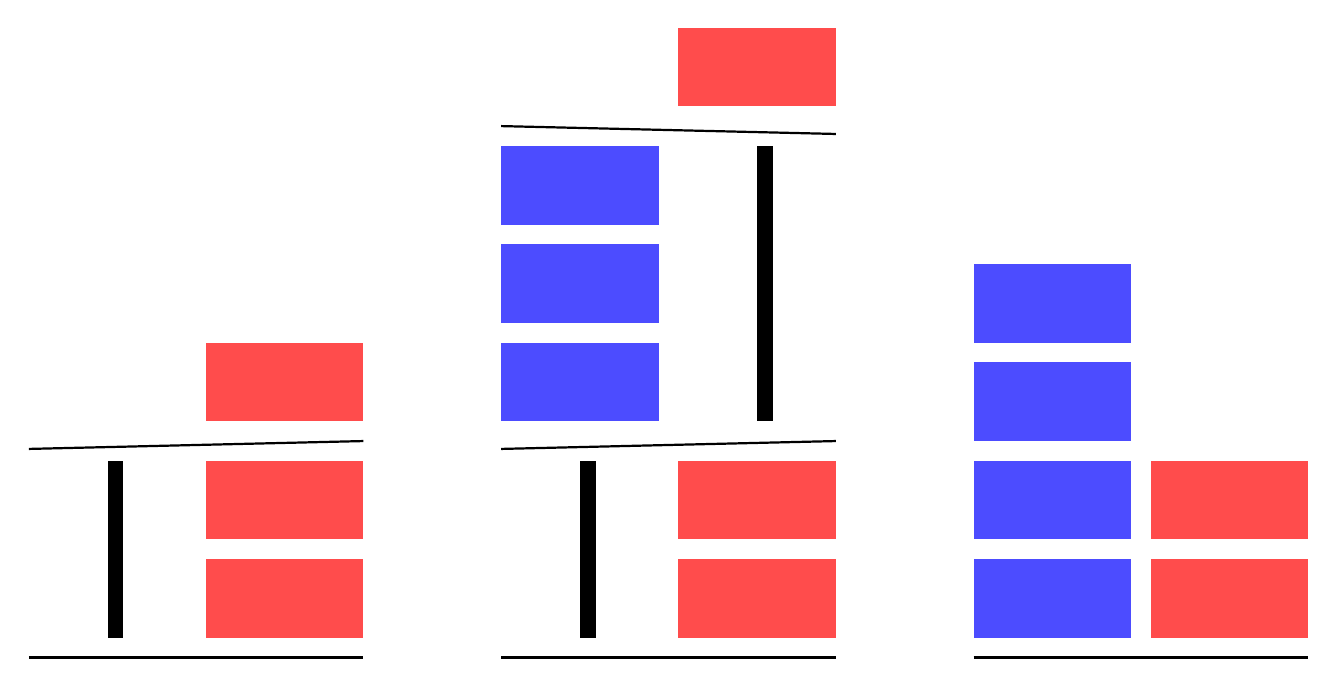
\begin{tikzpicture}
     
\draw[thick,black] (0,0) -- (4.25,0);
 
	\fill[red!70] (2.25,0.25) rectangle (4.25,1.25);
	\fill[red!70] (2.25,1.5) rectangle (4.25,2.5);
	
	\fill[black] (1,0.25) rectangle (1.2,2.5);
	 
\draw[thick,black] (0,2.65) -- (4.25,2.75);

	\fill[red!70] (2.25,3) rectangle (4.25,4);
	
\draw[thick,black] (6,0) -- (10.25,0);
 
	\fill[black] (7,0.25) rectangle (7.2,2.5);
	
	\fill[red!70] (8.25,0.25) rectangle (10.25,1.25);
	\fill[red!70] (8.25,1.5) rectangle (10.25,2.5);
	 
\draw[thick,black] (6,2.65) -- (10.25,2.75);

	\fill[blue!70] (6,3) rectangle (8,4);
	\fill[blue!70] (6,4.25) rectangle (8,5.25);
	\fill[blue!70] (6,5.5) rectangle (8,6.5);
 
	\fill[black] (9.25,3) rectangle (9.45,6.5);
	
\draw[thick,black] (6,6.75) -- (10.25,6.65);

	\fill[red!70] (8.25,7) rectangle (10.25,8);
	
\draw[thick,black] (12,0) -- (16.25,0);

	\fill[blue!70] (12,0.25) rectangle (14,1.25);
	\fill[blue!70] (12,1.5) rectangle (14,2.5);
	\fill[blue!70] (12,2.75) rectangle (14,3.75);
	\fill[blue!70] (12,4) rectangle (14,5);
	
	\fill[red!70] (14.25,0.25) rectangle (16.25,1.25);
	\fill[red!70] (14.25,1.5) rectangle (16.25,2.5);
    \end{tikzpicture}

\end{document}